\documentclass[xcolor={dvipsnames,table}]{beamer}
\usepackage{tikz}                   
\usetikzlibrary{shadows}
\usetheme{Dresden}
\usepackage[utf8]{inputenc}
\usepackage{polski}
\setbeamertemplate{blocks}[rounded][shadow=true]
\setbeamertemplate{footline}[frame number]
\usepackage{booktabs}
\usepackage{listings}
\usepackage{color}
 
\definecolor{codegreen}{rgb}{0,0.6,0}
\definecolor{codegray}{rgb}{0.5,0.5,0.5}
\definecolor{codepurple}{rgb}{0.58,0,0.82}
\definecolor{backcolour}{rgb}{0.95,0.95,0.92}
 
\lstdefinestyle{mystyle}{
    backgroundcolor=\color{backcolour},   
    commentstyle=\color{codegreen},
    keywordstyle=\color{magenta},
    numberstyle=\tiny\color{codegray},
    stringstyle=\color{codepurple},
    basicstyle=\footnotesize,
    breakatwhitespace=false,         
    breaklines=true,                 
    captionpos=b,                    
    keepspaces=true,                 
    numbers=left,                    
    numbersep=5pt,                  
    showspaces=false,                
    showstringspaces=false,
    showtabs=false,                  
    tabsize=2
}
 
\lstset{style=mystyle}
%Information to be included in the title page:
\title{Programowanie sprzętu w laboratorium fotoniki}
\author{Paweł Gliwny}
\institute{Instytut Fizyki \\ Politechnika Łódzka}
\date{2017}
 
 
 
\begin{document}


\frame{\titlepage}

\begin{frame}
\begin{Large}
\begin{center}
,,Mówca powinien wyczerpać temat, ale w żadnym razie nie powinien wyczerpać publiczności" --- Winston Churchill
\end{center}
\end{Large}
\end{frame}

\begin{frame}
\frametitle{Plan}
\begin{enumerate}
\item Cel pracy.
\item Układ pomiarowy.
\item Eksperyment.
\end{enumerate}
\end{frame}

\begin{frame}
\begin{Huge}
\begin{center}
Cel pracy
\end{center}
\end{Huge}
\end{frame}

\begin{frame}
\frametitle{Cel pracy}
\begin{itemize}
\item Stworzenie programu do wykonywania charakterystyk laserów półprzewodnikowych.
\item Wykonanie przykładowej charakterystyki
\end{itemize}
\end{frame}

\begin{frame}
\begin{Huge}
\begin{center}
Układ pomiarowy.
\end{center}
\end{Huge}
\end{frame}

\begin{frame}
\frametitle{Układ pomiarowy}
\begin{itemize}
\item Zasilacza diód laserowych firmy Thorlabs model LDC4005 
\begin{figure}
%\hspace{4cm}  \vspace{1cm}
   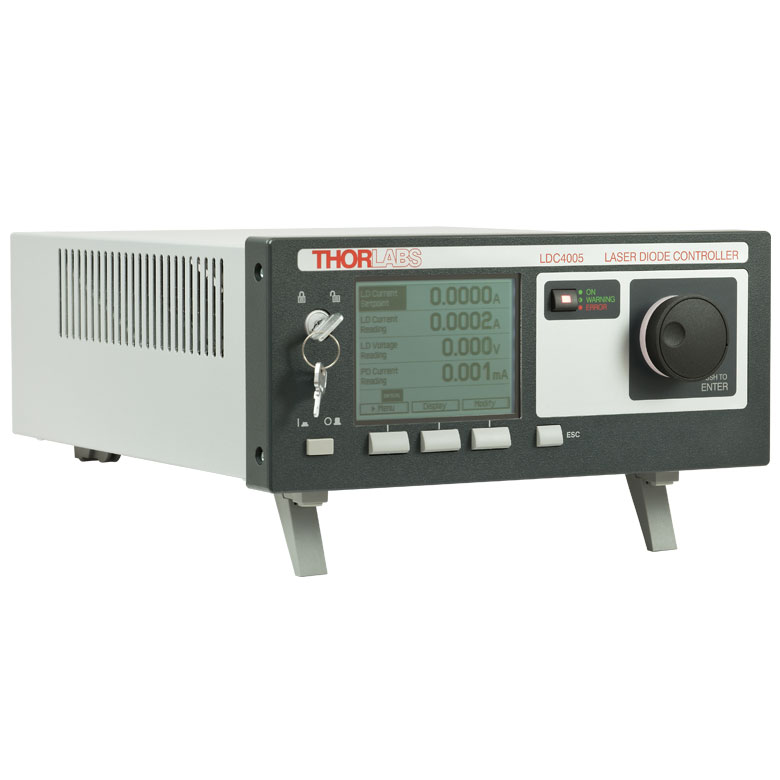
\includegraphics[width=0.35\textwidth,natwidth=69,natheight=87]{ldc4005.jpg}
\end{figure}
\item Miernik mocy firmy Thorlas firmy Thorlabs model PM100
\begin{figure}
%\hspace{4cm}  \vspace{1cm}
   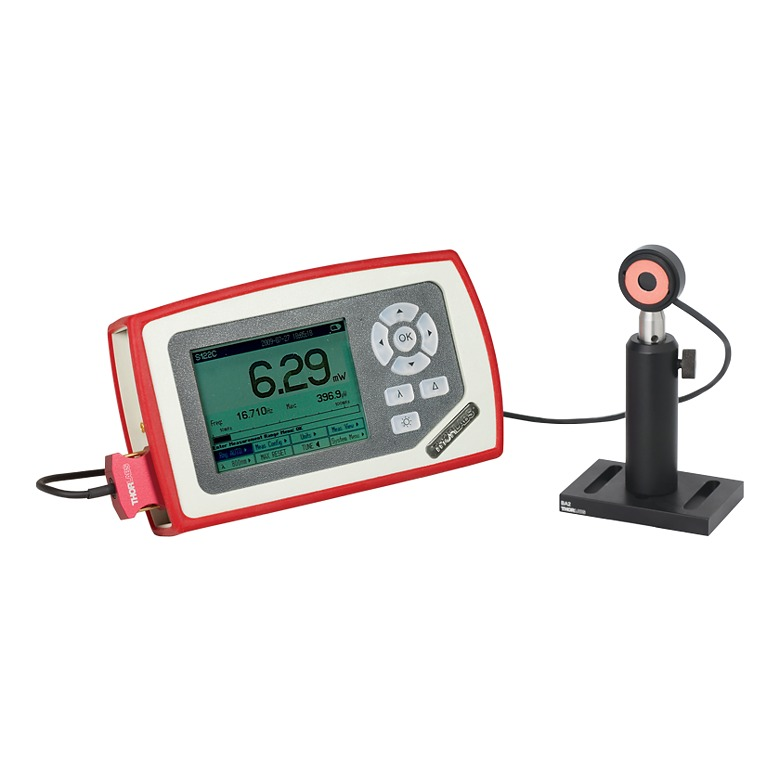
\includegraphics[width=0.35\textwidth,natwidth=69,natheight=87]{pm100.jpg}
\end{figure}
\end{itemize}
\end{frame}


\begin{frame}
\frametitle{Programowane urządzenia pomiarowe}
Electronic test equipment --- są używane w celu przechywywania sygnałów oraz podawanie ich do sprzętu
\end{frame}

\begin{frame}
\frametitle{Komunikacja z urządzenimi}
\begin{itemize}
\item SCPI (ang. Standard Commands for Programmable Instruments) --- język komend do urządzeń pomiarowych.
\item Wywołania systemowe (ang. System call)
\end{itemize}
SCPI + Wywołania systemowe = komunikacja z sprzętem laboratoryjnym
\end{frame}

\begin{frame}
\frametitle{SCPI --- Standard Commands for Programmable Instruments}
Standardowe polecenia programowanych urządzeń jest to standard komunikacji
\begin{itemize}
\item z urządzeniami pomiarowymi (oscyloskop, miernik mocy).
\item z urządzeniami laboratoryjnymi (zasiłacz)
\end{itemize} 
\end{frame}

\begin{frame}
\frametitle{SCPI --- przykłady}
\begin{itemize}
\item Komendy uniwersalne dla każdego urządzenia:
\begin{itemize}
\item $\mathtt{*rst}$ --- wyzerowanie urządzenia.
\item $\mathtt{*idn?}$ --- zapytanie o identyfikator.
\end{itemize}
\item Komendy specyficzny dla danego urządzenia:
\begin{itemize}
\item $\mathtt{SOURce:CURRent:LEVel:AMPLitude}$  $\mathtt{0.01}$
\end{itemize}
\end{itemize}
\end{frame}

\begin{frame}
\frametitle{Wywołania systemowe}
Interfejs pomiędzy programem użytkownika a jądrem Linux.
\begin{itemize}
\item $\mathtt{open}$.
\item $\mathtt{write}$.
\item $\mathtt{read}$.
\item $\mathtt{close}$.
\end{itemize}
\end{frame}

\begin{frame}
\frametitle{Przykładowy program}
\lstinputlisting[language=Python, firstline=0, lastline=20]{deviceio.py}
\end{frame}

\begin{frame}
\begin{Huge}
\begin{center}
Eksperyment
\end{center}
\end{Huge}
\end{frame}

\begin{frame}
\frametitle{Teoria --- prąd progowy}
Prąd progowy (z ang. \textit{threshold current}) określa wartość prądu przy którym zaczyna zachodzić akcja laserowa czyli rośnie gwałtownie natężenie promieniowania i maleje szerokość linii emisyjnej.
\begin{figure}
%\hspace{4cm}  \vspace{1cm}
   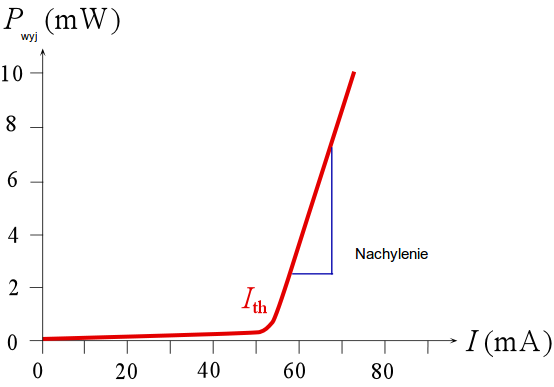
\includegraphics[width=0.65\textwidth,natwidth=69,natheight=87]{slope.png}
\end{figure}
\end{frame}

\begin{frame}
\frametitle{Prąd progowy zależność od temperatury}

\begin{equation*}
I_{th} = I_0 \exp \left( \frac{T}{T_0} \right)
\end{equation*}

\begin{equation*}
\ln (I_{th}) =  \ln \left( \frac{T}{T_0} \right) + \ln(I_{0})
\end{equation*}

\begin{equation*}
y = a \cdot x + b
\end{equation*}

\begin{equation*}
a = \frac{1}{T_0} \Rightarrow T_0 = \frac{1}{a}
\end{equation*}

\begin{equation*}
b = \ln(I_0) \Rightarrow I_0 = e^b
\end{equation*}
\end{frame}

\begin{frame}
\frametitle{Sprawność}
\begin{itemize}
\item Moc wyjściowa  ---  mierzymy na mierniku mocy.
\item Moc wejściowa --- iloczyn prądu $I$ i napięcia $U$.
\begin{equation*}
P_{in} = I \cdot U
\end{equation*}
\end{itemize}
\end{frame}

\begin{frame}
\center
\begin{figure}
%\hspace{4cm}  \vspace{1cm}
   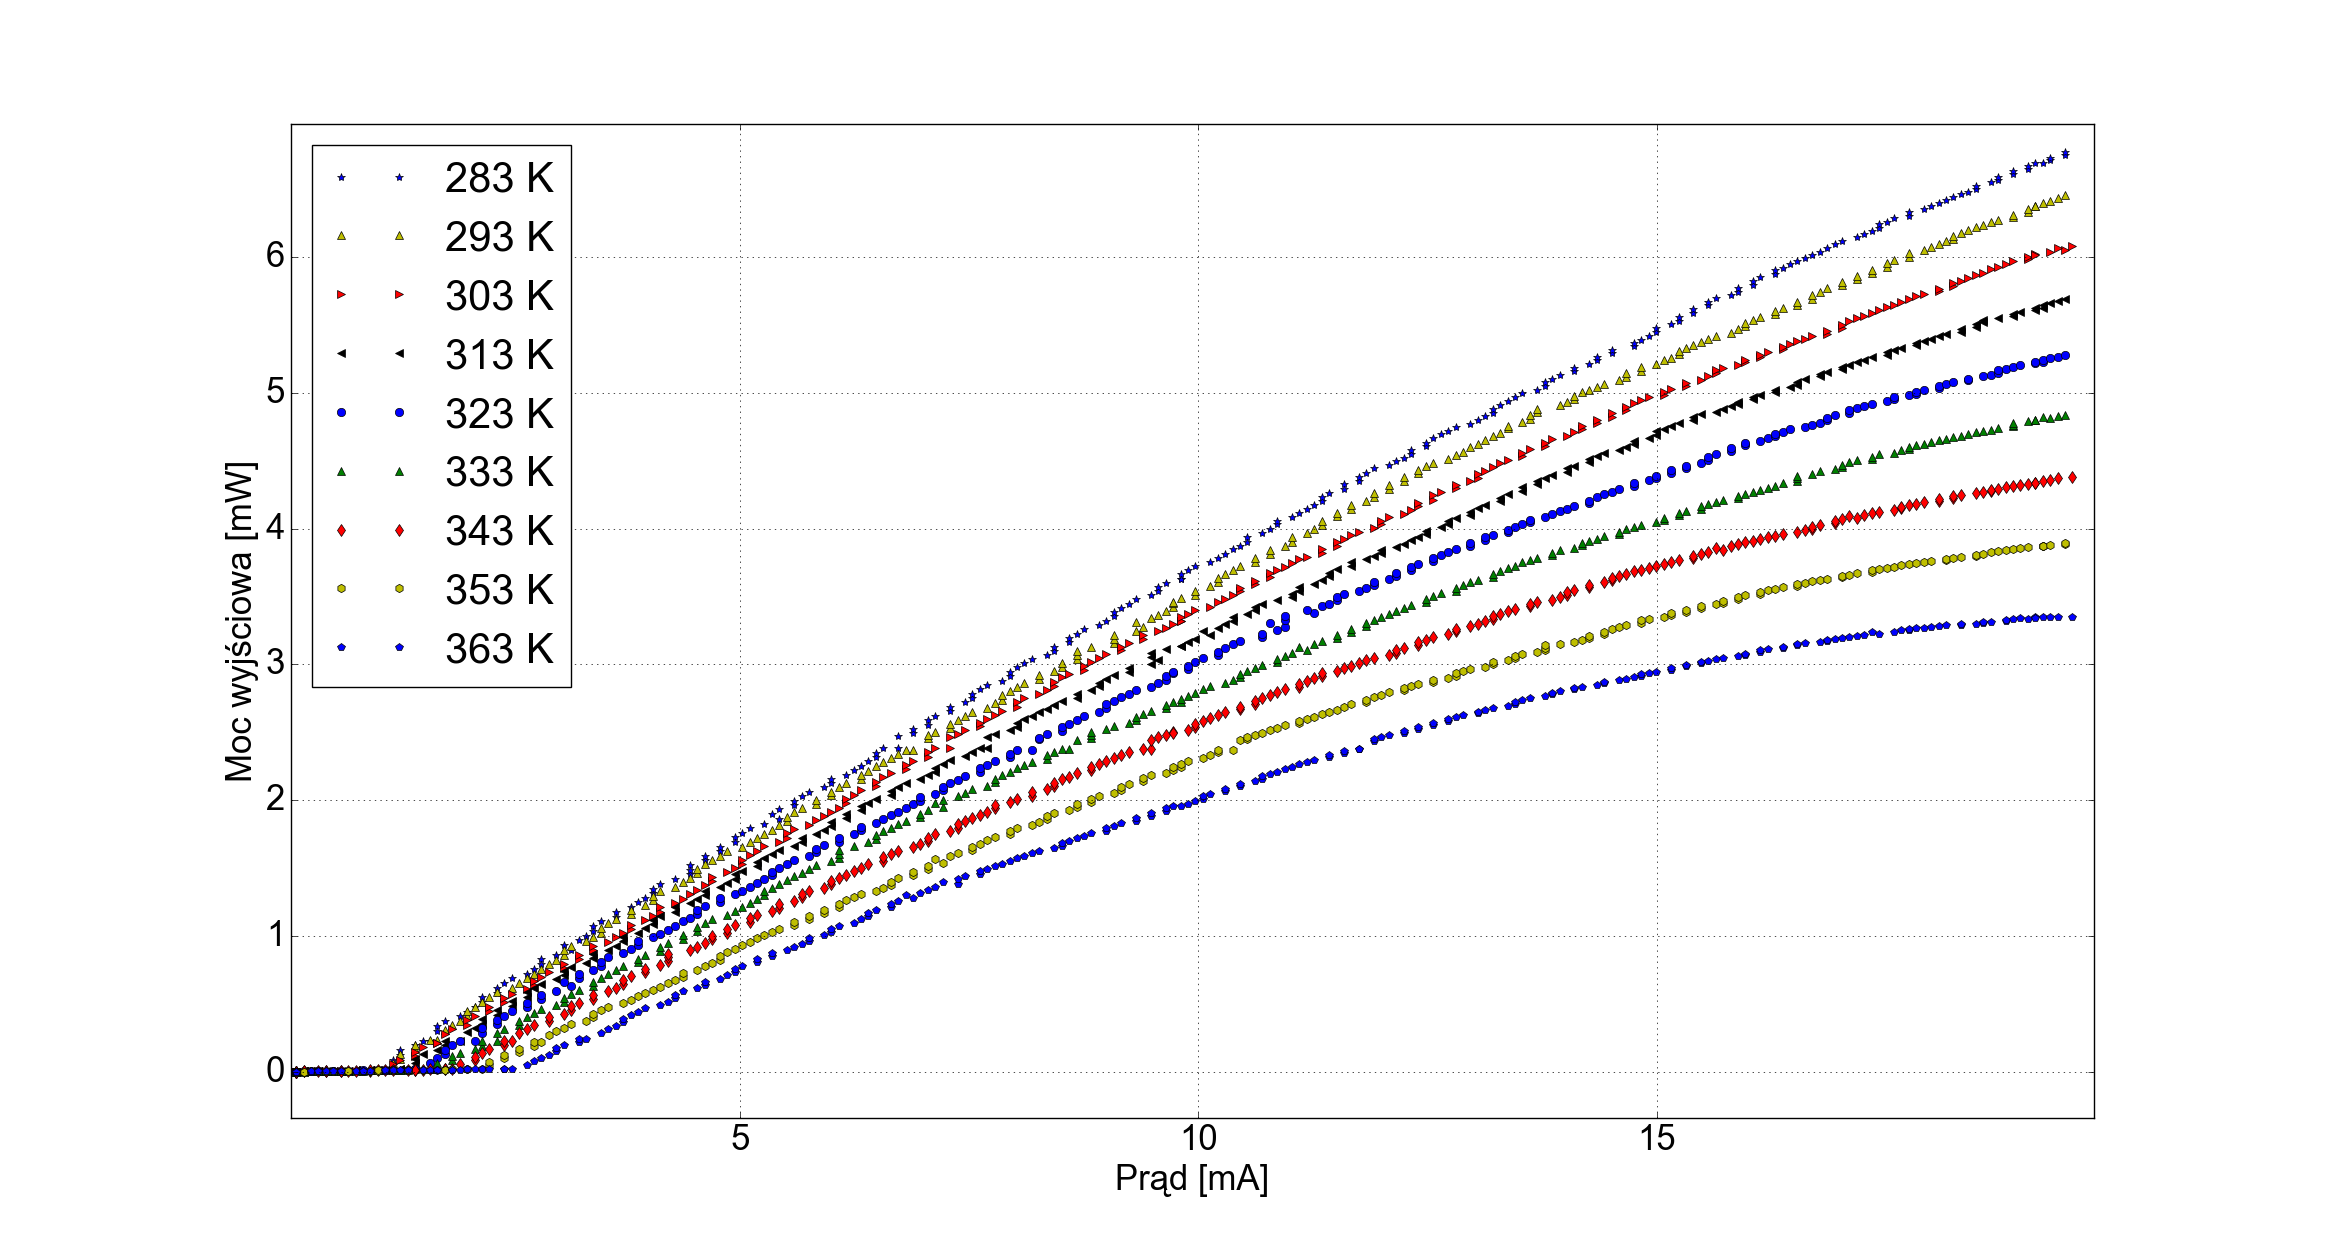
\includegraphics[width=1.10\textwidth,natwidth=69,natheight=87]{plot_all.png}
\end{figure}

\end{frame}


\begin{frame}
\center
\begin{figure}
%\hspace{4cm}  \vspace{1cm}
   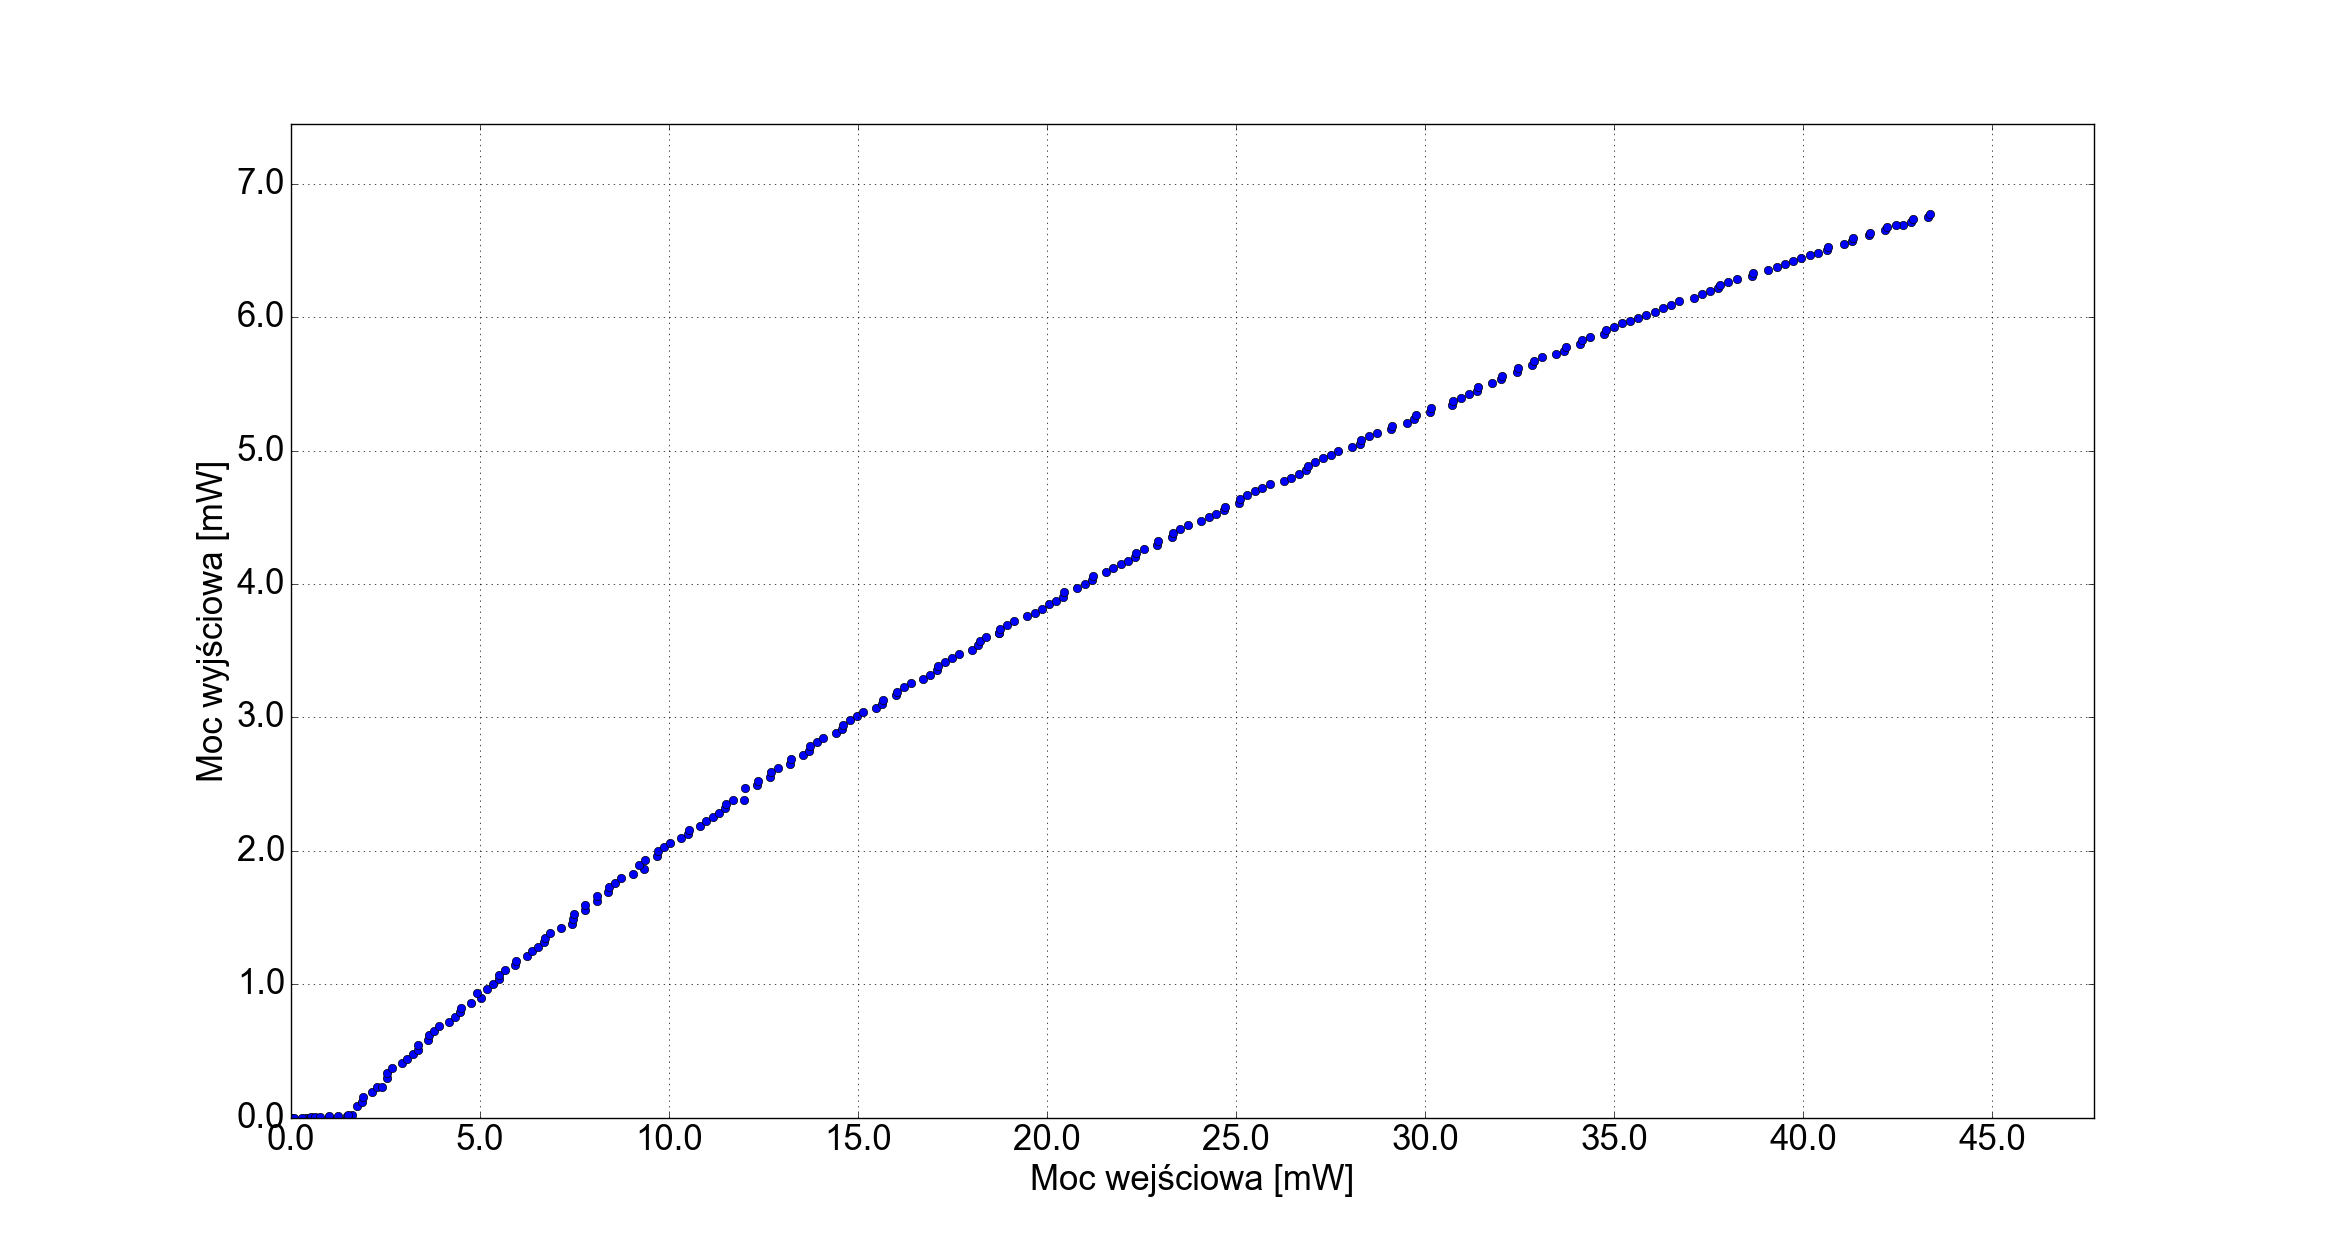
\includegraphics[width=1.10\textwidth,natwidth=69,natheight=87]{temp_10_power.png}
\end{figure}

\end{frame}

\begin{frame}
\center
\begin{figure}
%\hspace{4cm}  \vspace{1cm}
   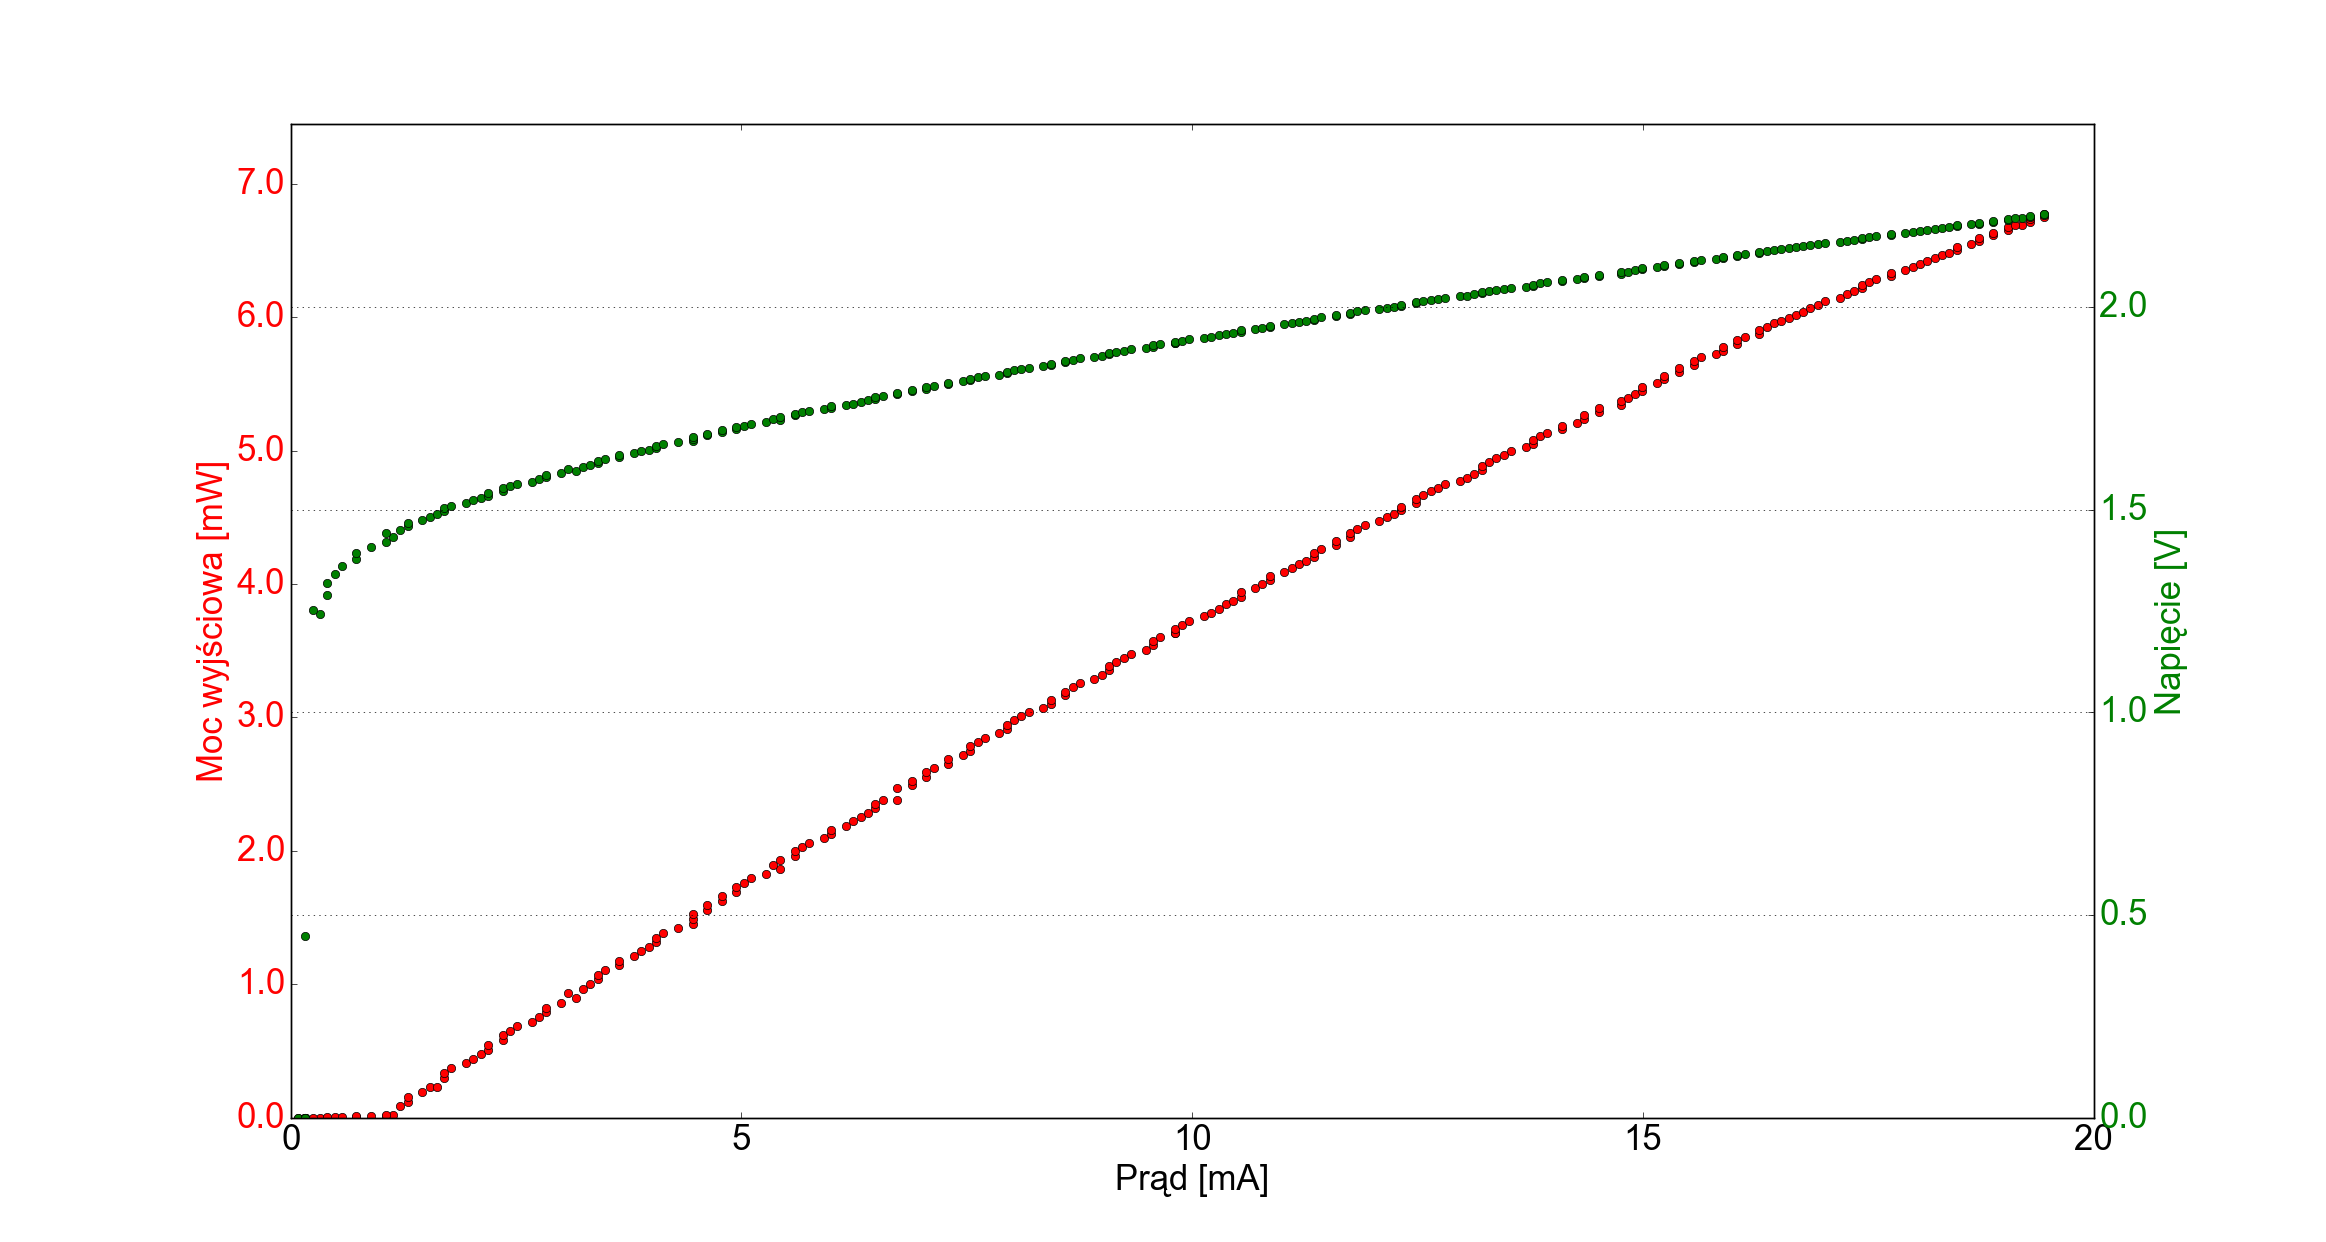
\includegraphics[width=1.10\textwidth,natwidth=69,natheight=87]{temp_10_IVL.png}
\end{figure}

\end{frame}


\begin{frame}
\center
\begin{figure}
%\hspace{4cm}  \vspace{1cm}
   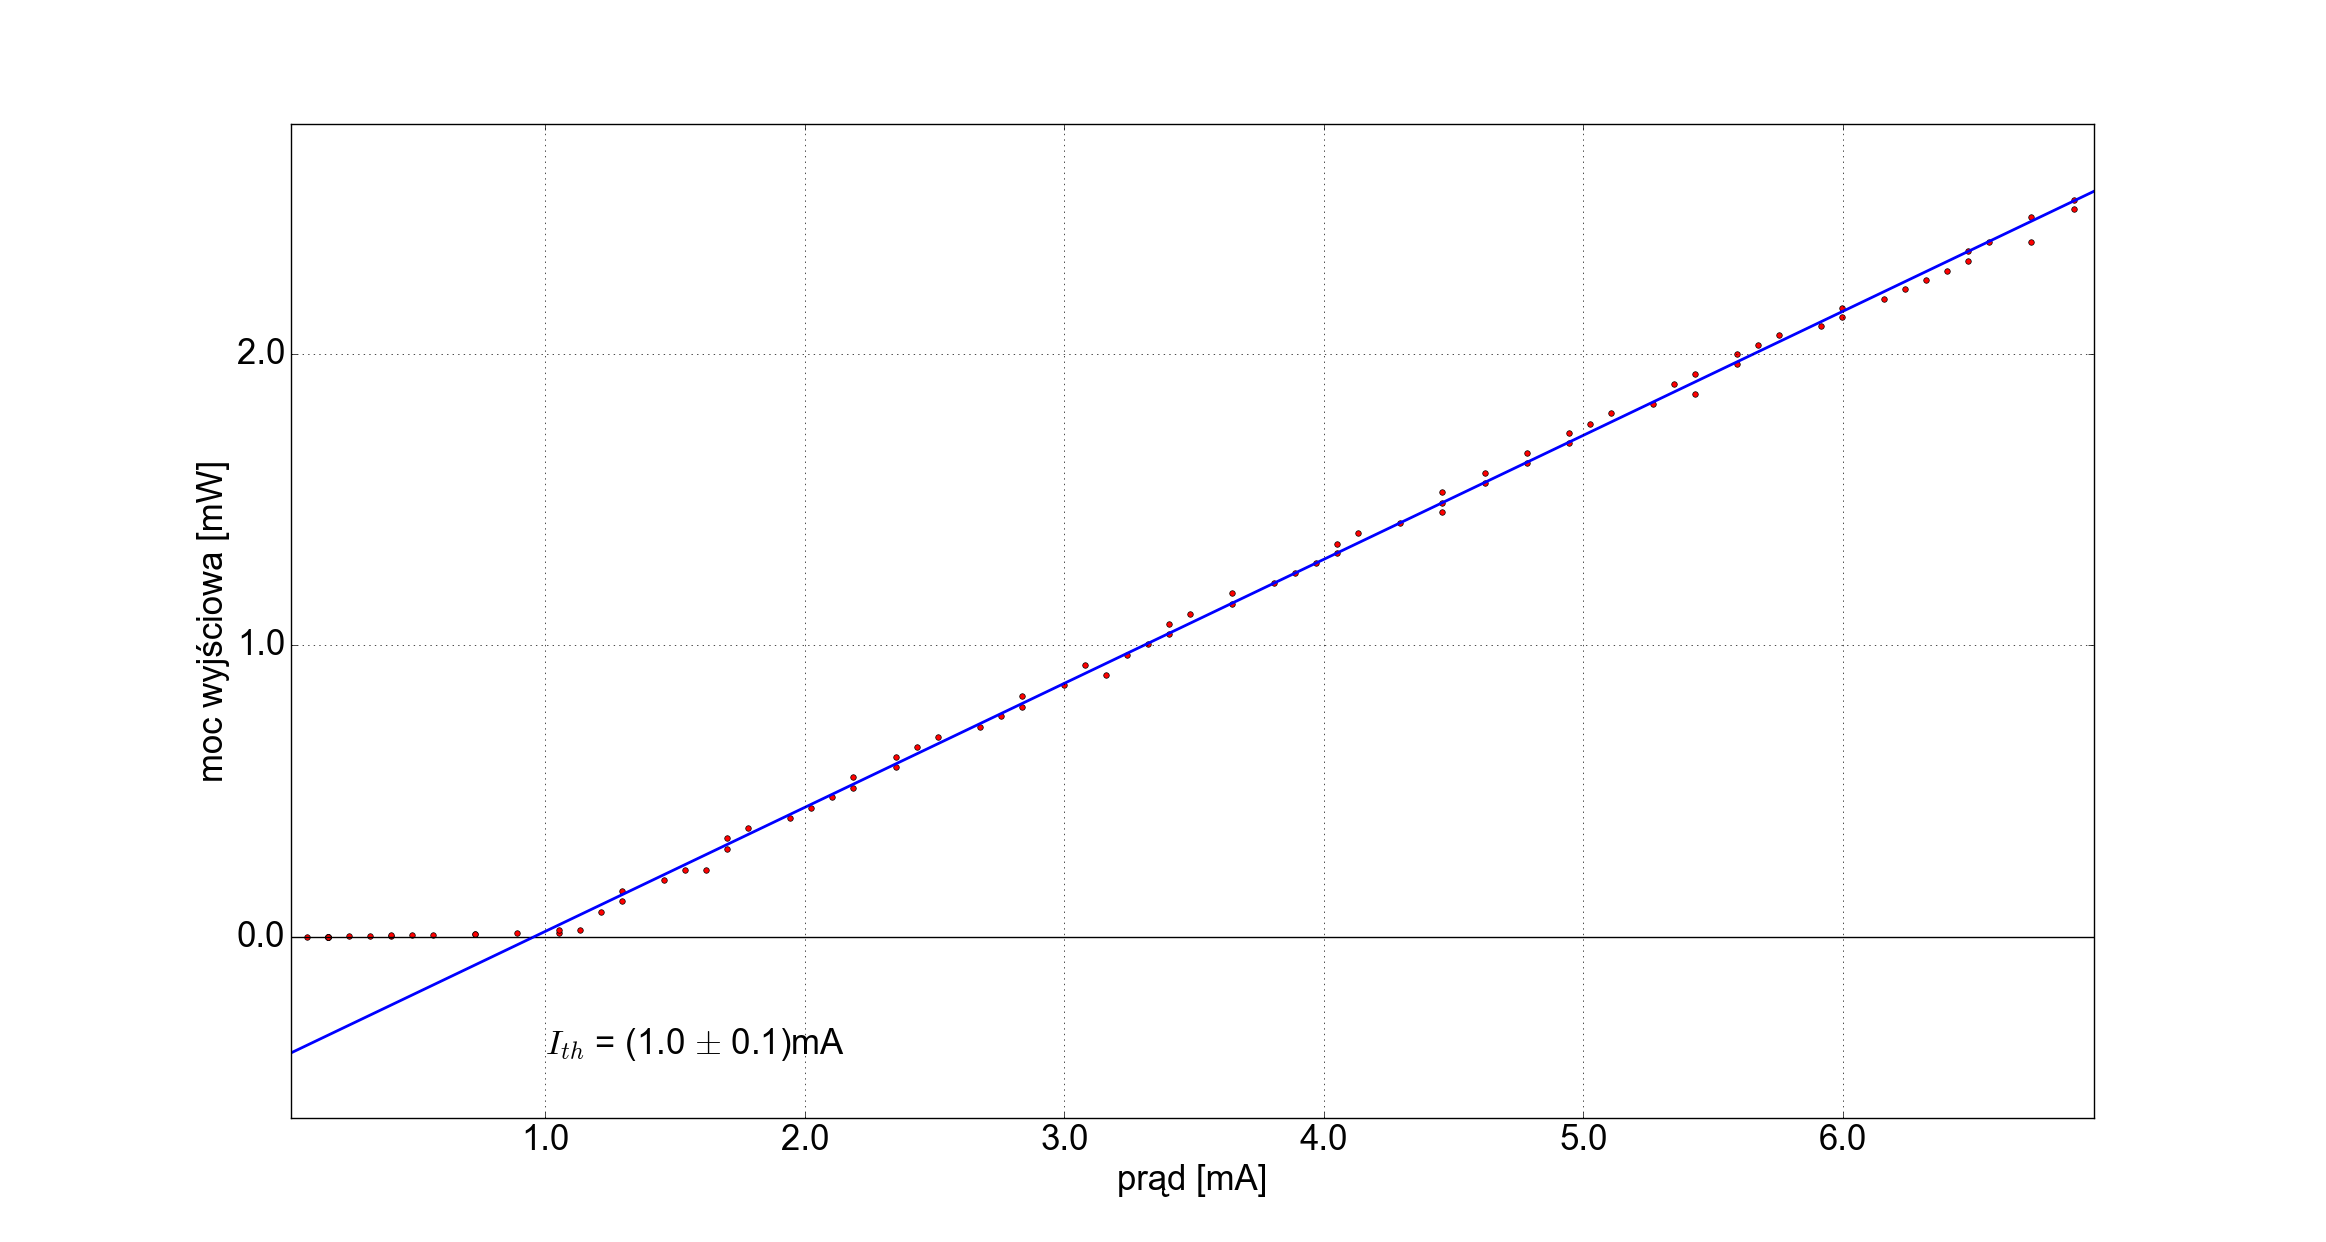
\includegraphics[width=1.10\textwidth,natwidth=69,natheight=87]{temp_10_fit.png}
\end{figure}
\end{frame}

\begin{frame}
\center
\begin{figure}
%\hspace{4cm}  \vspace{1cm}
   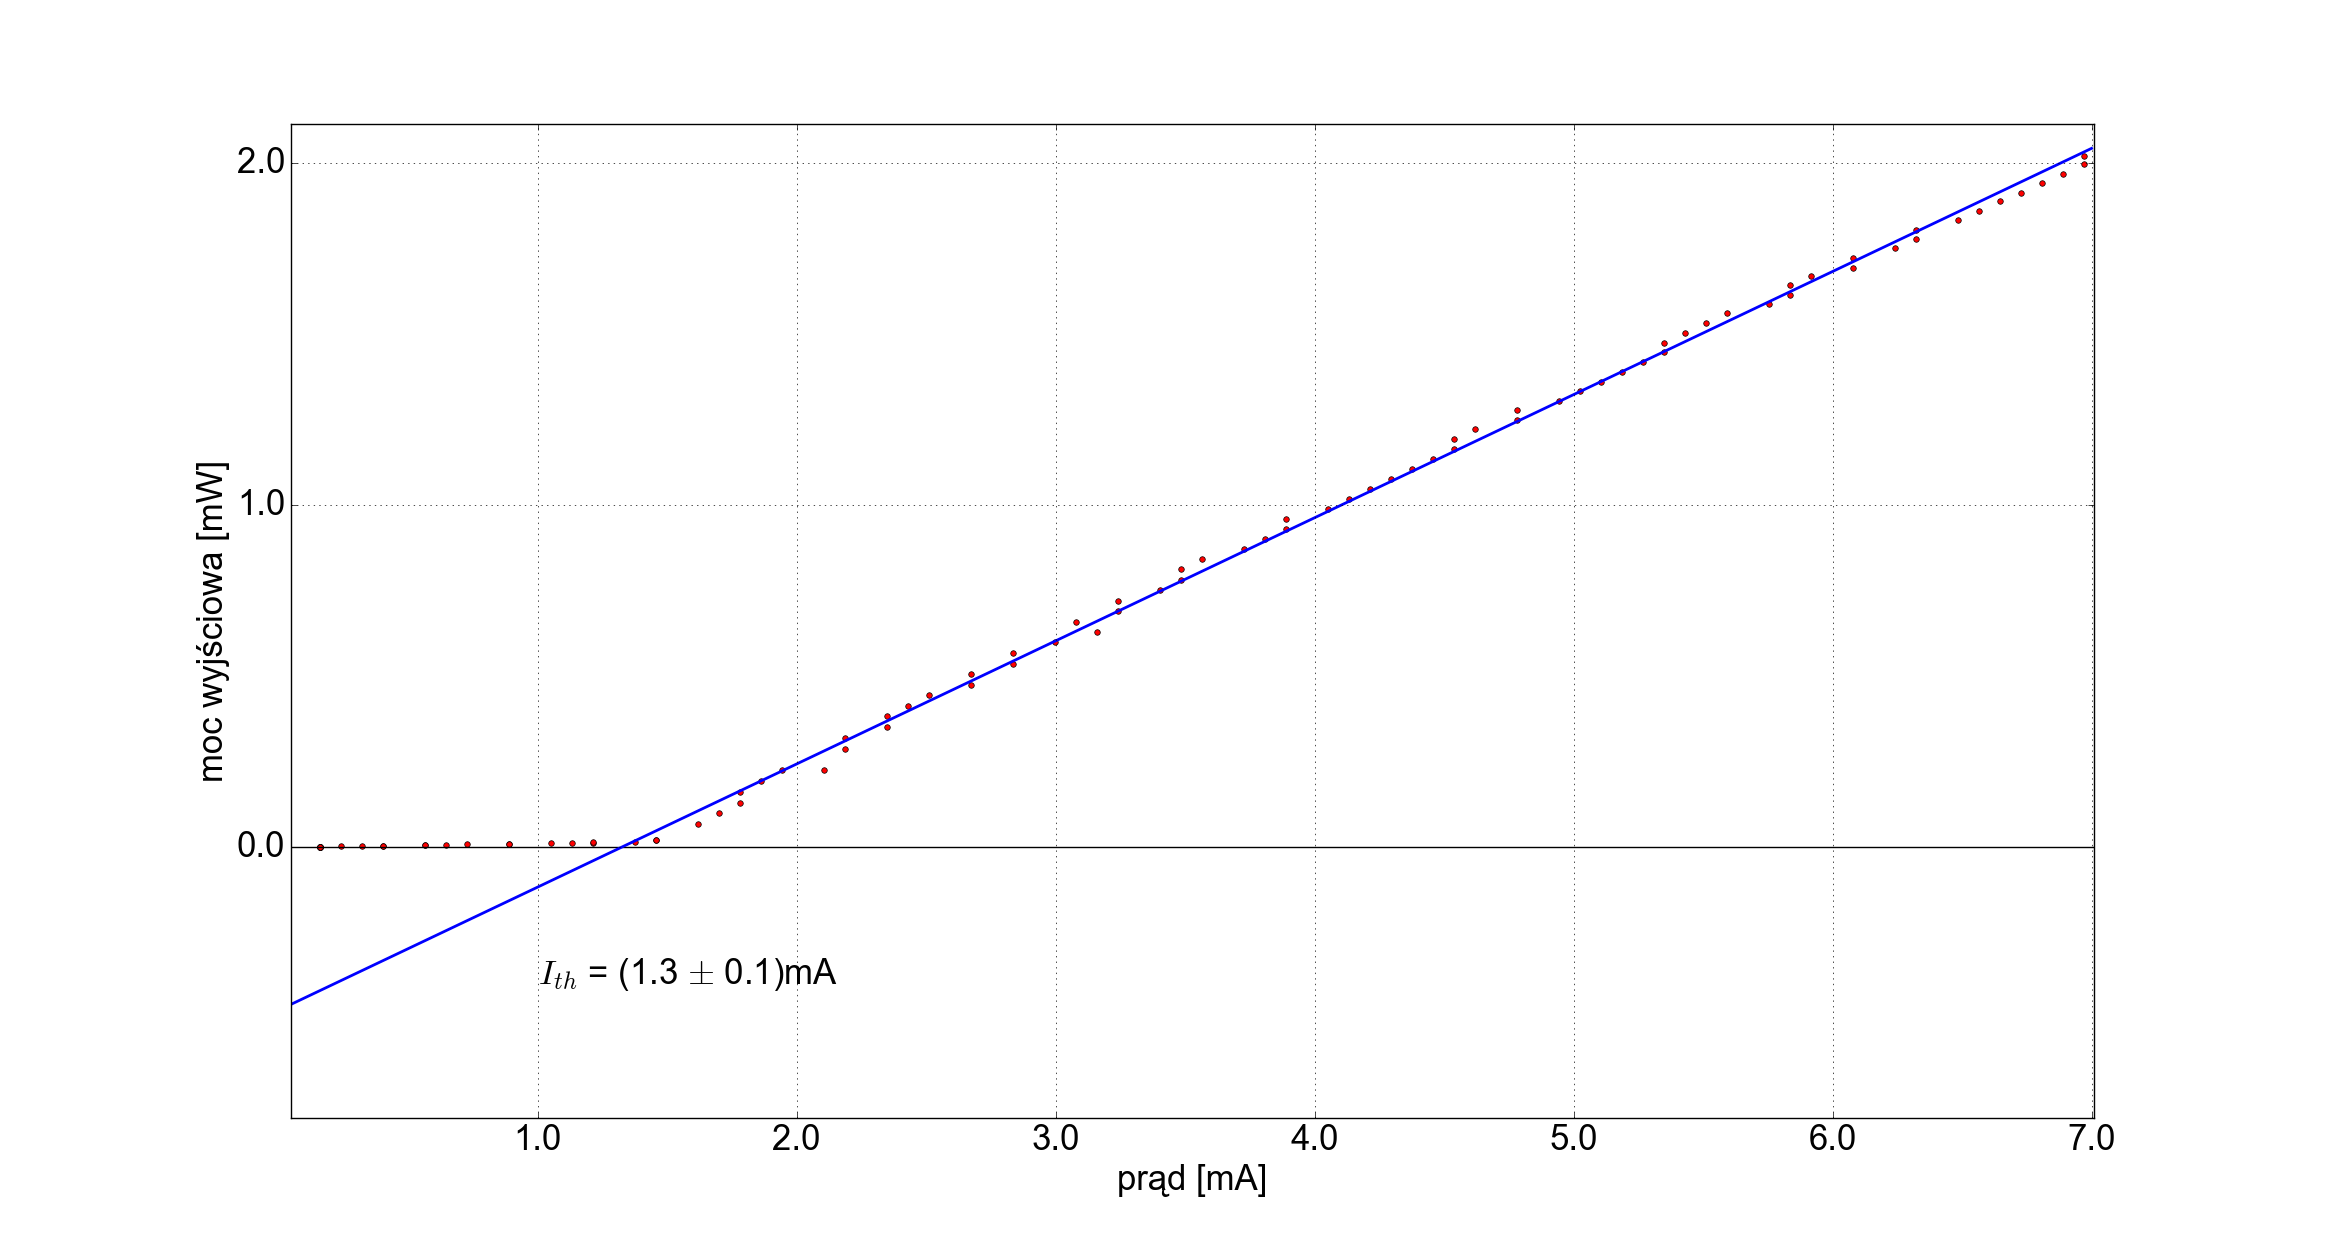
\includegraphics[width=1.10\textwidth,natwidth=69,natheight=87]{temp_50_fit.png}
\end{figure}
\end{frame}

\begin{frame}
\center
\begin{figure}
%\hspace{4cm}  \vspace{1cm}
   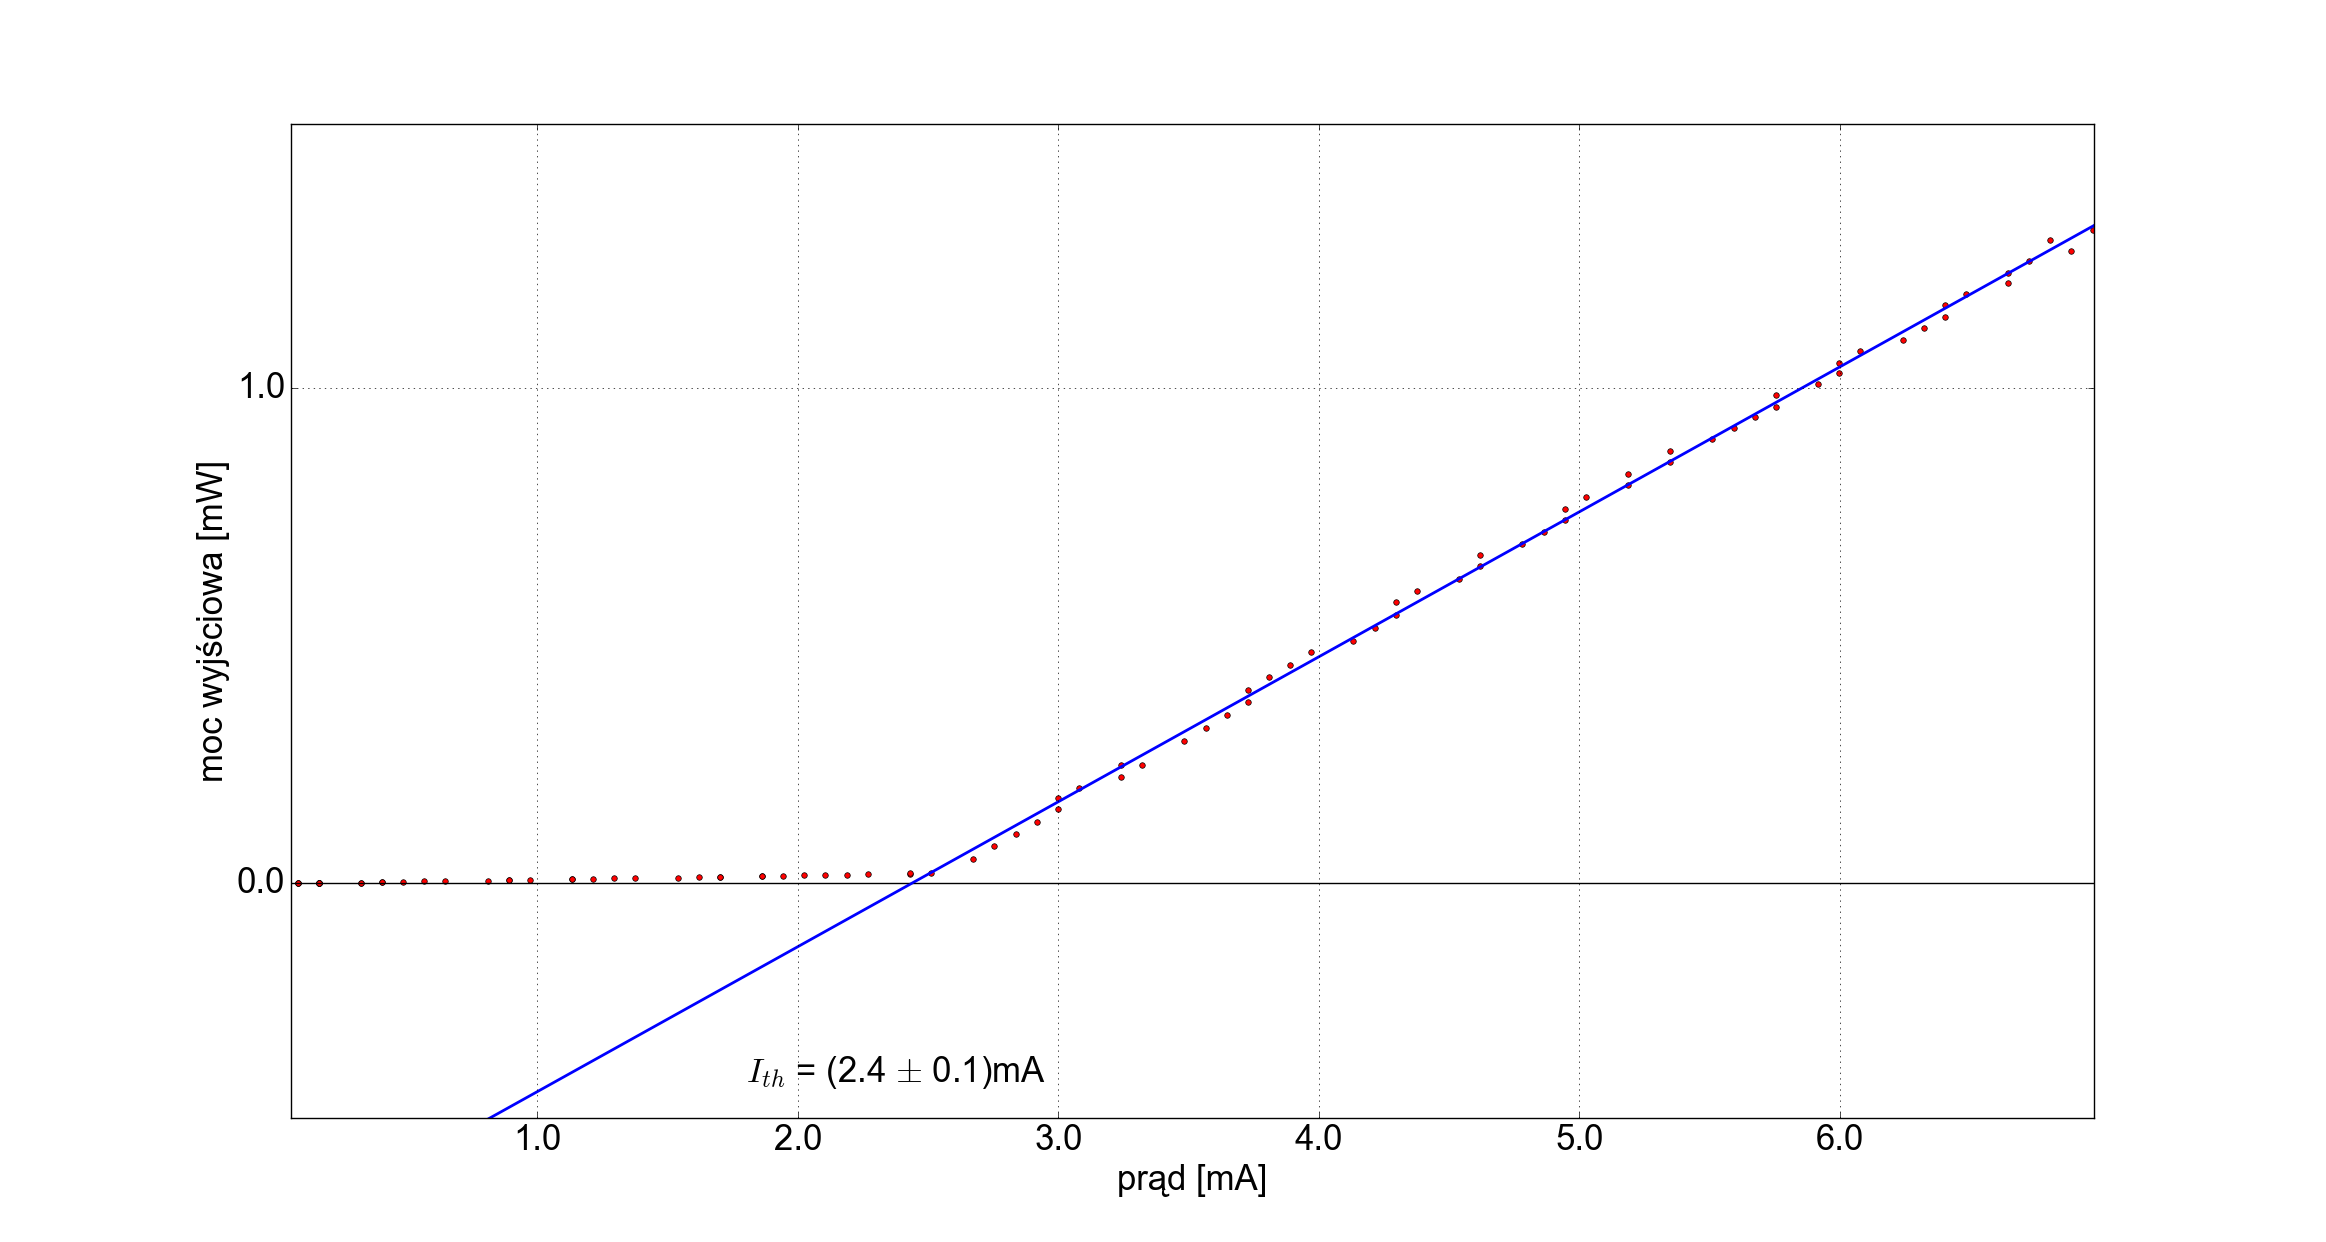
\includegraphics[width=1.10\textwidth,natwidth=69,natheight=87]{temp_90_fit.png}
\end{figure}
\end{frame}

\begin{frame}
\center
\begin{figure}
%\hspace{4cm}  \vspace{1cm}
   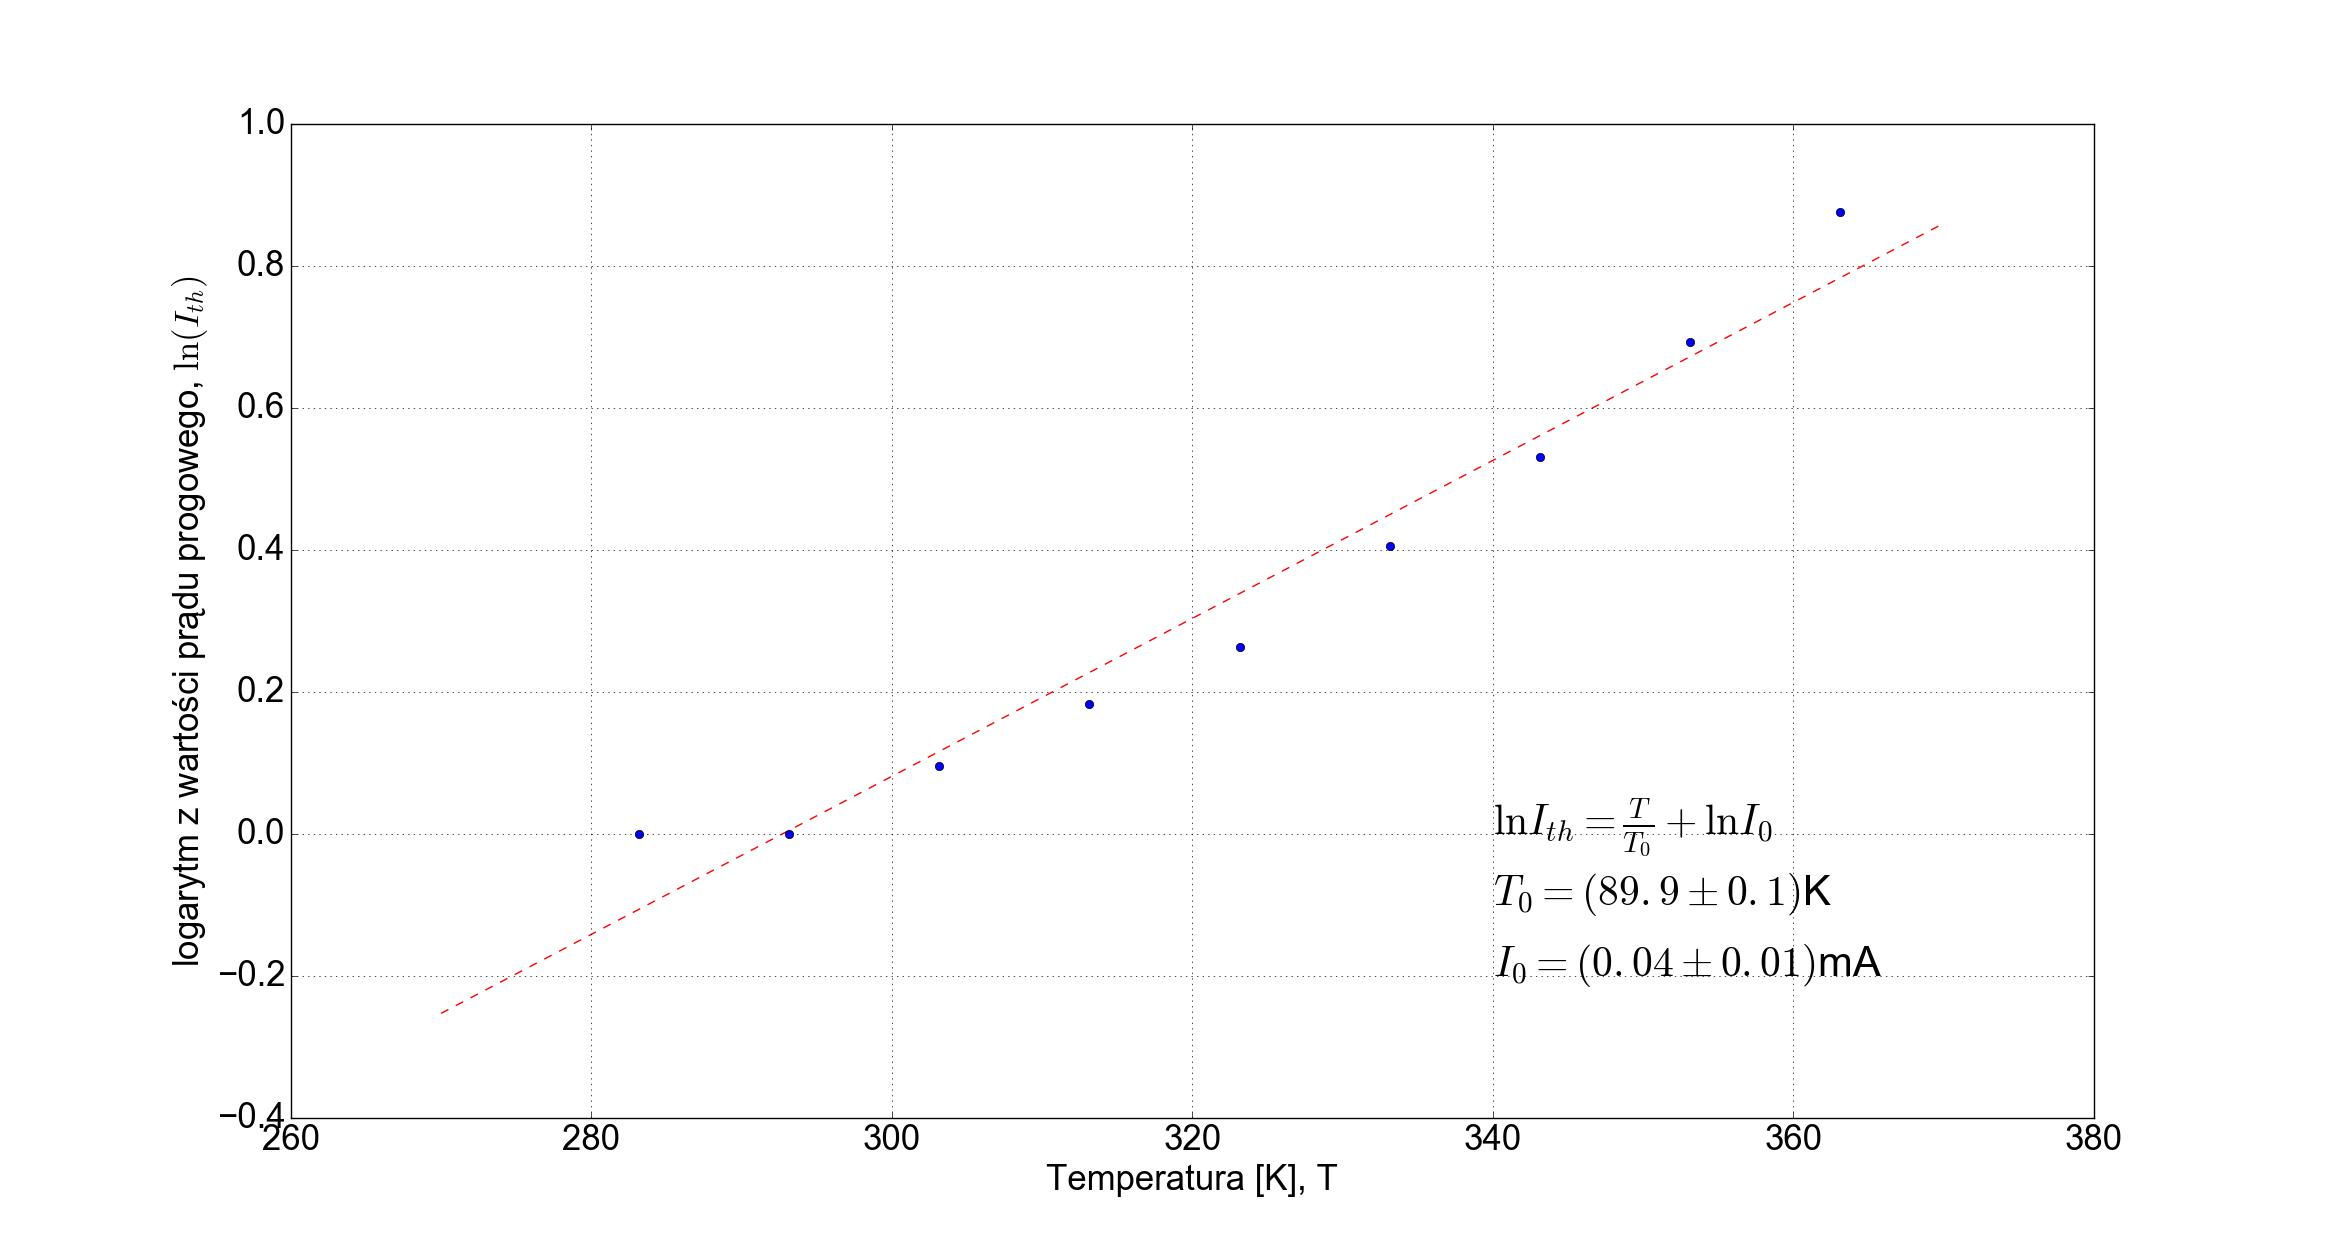
\includegraphics[width=1.10\textwidth,natwidth=69,natheight=87]{fit_i_th.png}
\end{figure}
\end{frame}

\begin{frame}
\frametitle{Laser krawędziowy 980\,nm}
\begin{itemize}
\item $T_0 = (89.9 \pm 0.1)$\,K
\item $I_0 = (0.04 \pm 0.01)$\,mA
\end{itemize}
\begin{equation*}
I_{th} = 0.04 \exp \left( \frac{T}{89.9} \right)
\end{equation*}
\end{frame}

\begin{frame}
\frametitle{Laser krawędziowy 980\,nm}
\center
\begin{figure}
%\hspace{4cm}  \vspace{1cm}
   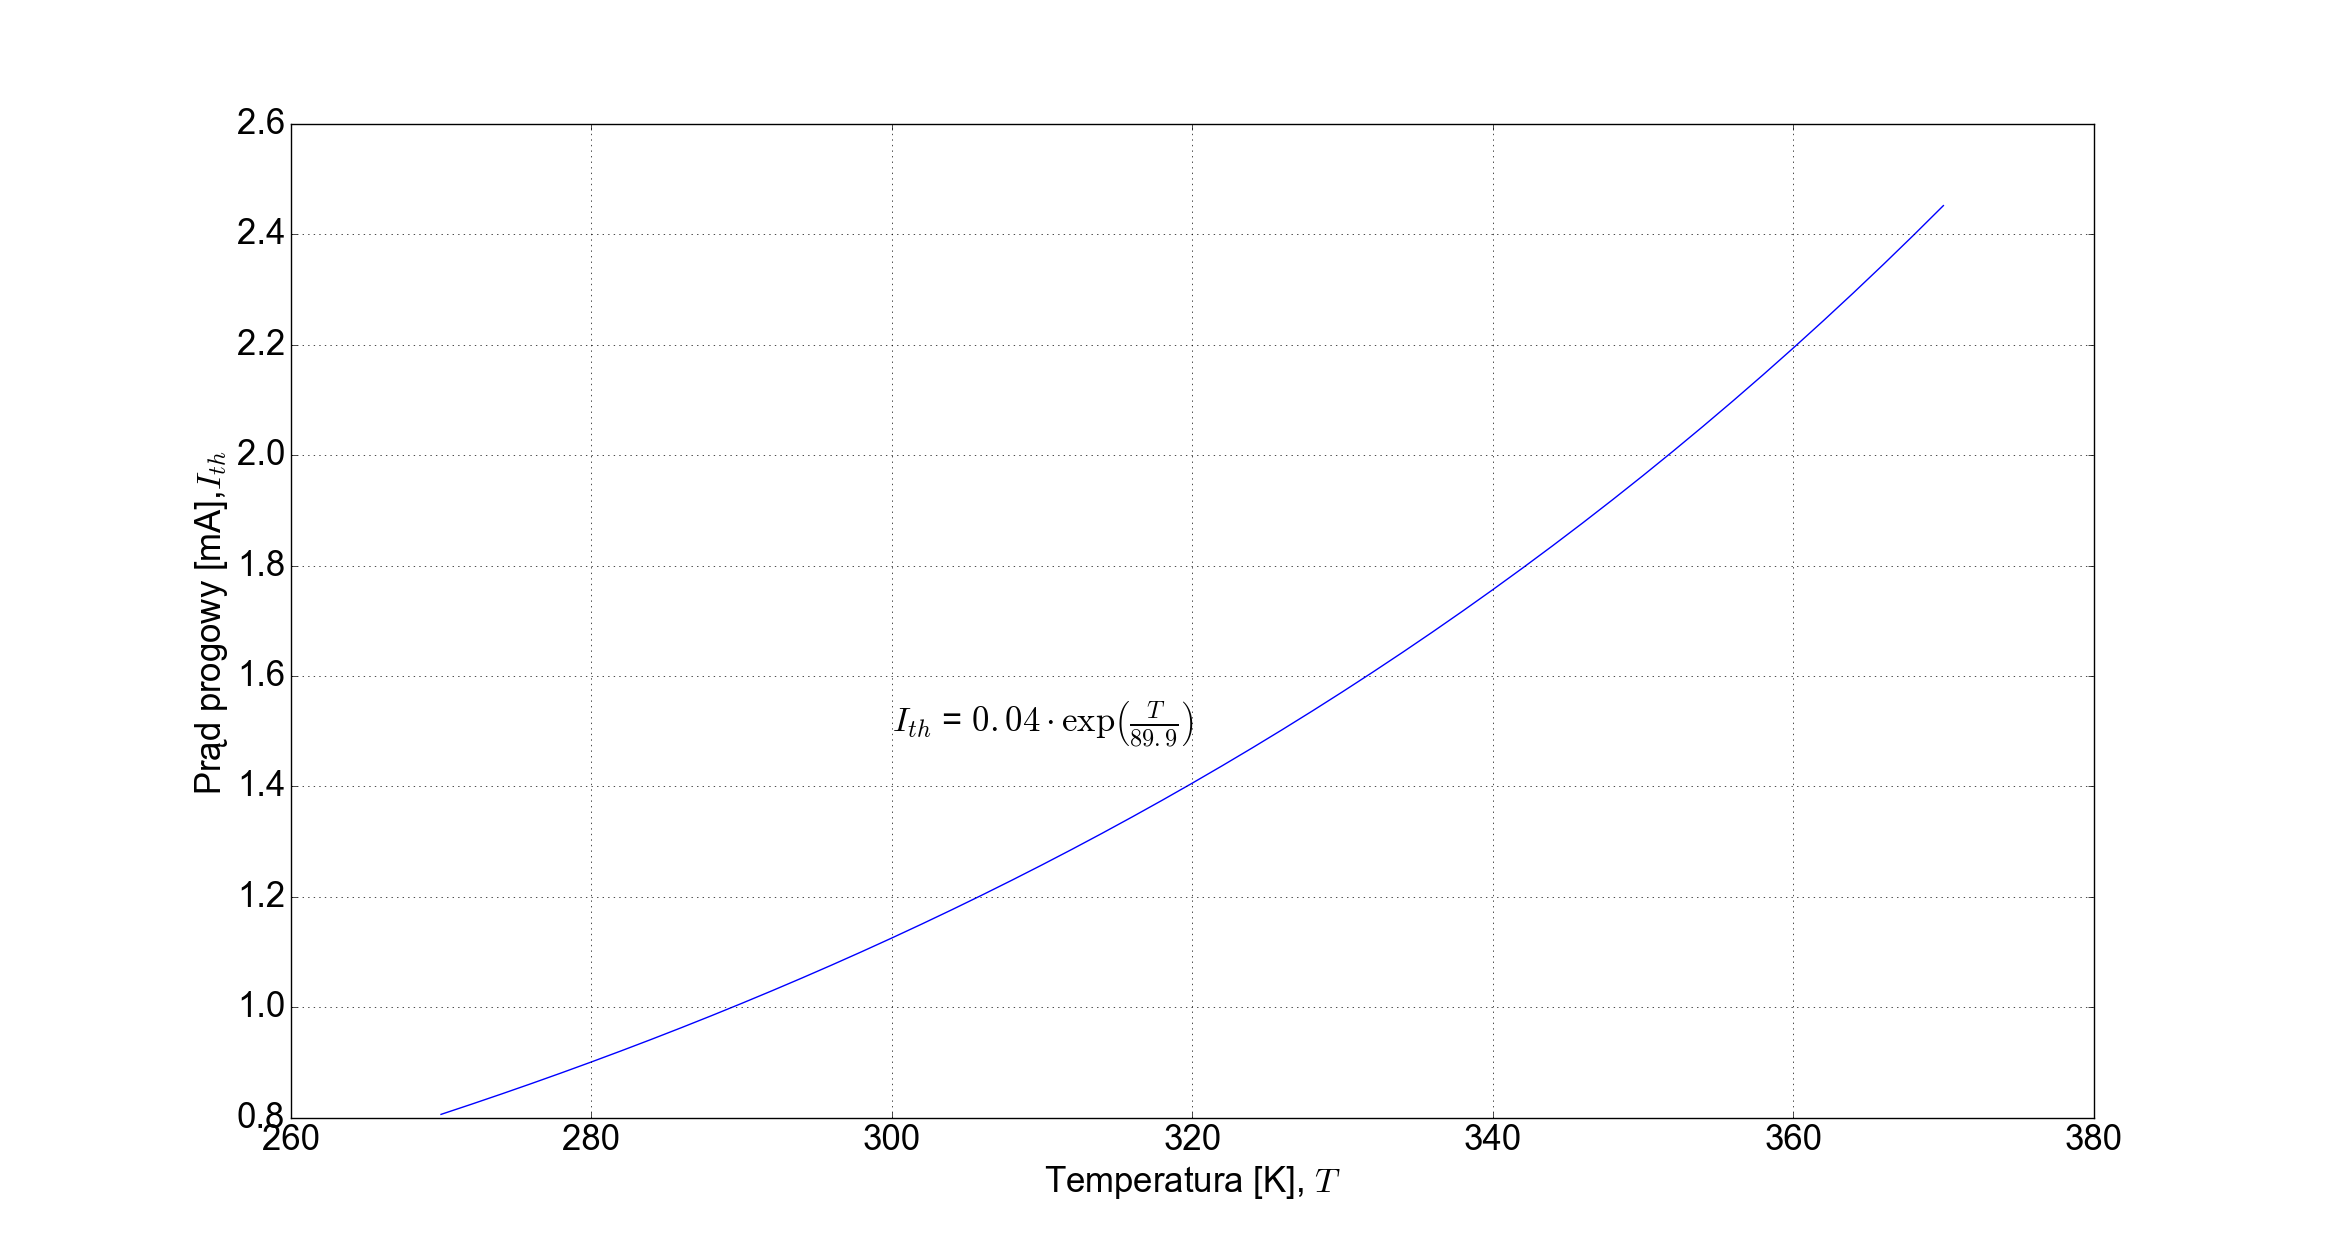
\includegraphics[width=1.10\textwidth,natwidth=69,natheight=87]{plot_i_th.png}
\end{figure}
\end{frame}

\end{document}